% Template from Springer
%
% First comes an example EPS file -- just ignore it and
% proceed on the \documentclass line
% your LaTeX will extract the file if required
% \begin{filecontents*}{example.eps}
% %!PS-Adobe-3.0 EPSF-3.0
% %%BoundingBox: 19 19 221 221
% %%CreationDate: Mon Sep 29 1997
% %%Creator: programmed by hand (JK)
% %%EndComments
% gsave
% newpath
%   20 20 moveto
%   20 220 lineto
%   220 220 lineto
%   220 20 lineto
% closepath
% 2 setlinewidth
% gsave
%   .4 setgray fill
% grestore
% stroke
% grestore
% \end{filecontents*}
%
\RequirePackage{fix-cm}
%
%\documentclass{svjour3}                     % onecolumn (standard format)
%\documentclass[smallcondensed]{svjour3}     % onecolumn (ditto)
\documentclass[smallextended]{svjour3}       % onecolumn (second format)
%\documentclass[twocolumn]{svjour3}          % twocolumn
%
\smartqed  % flush right qed marks, e.g. at end of proof
%
\usepackage{graphicx}
\usepackage{caption} % for subfigures
\usepackage{subcaption} % for subfigures
\usepackage{setspace, amsmath}
\usepackage{etoolbox} % for block quotes
\AtBeginEnvironment{quote}{\singlespacing\small} %for block quotes

\newcommand{\comm}[1]{}
%
% \usepackage{mathptmx}      % use Times fonts if available on your TeX system
%
% insert here the call for the packages your document requires
%\usepackage{latexsym}
% etc.
%
% please place your own definitions here and don't use \def but
% \newcommand{}{}
%
% Insert the name of "your journal" with
% \journalname{myjournal}
%
\begin{document}

\title{Predicting personality based on social media posts
}
%\subtitle{Do you have a subtitle?\\ If so, write it here}

%\titlerunning{Short form of title}        % if too long for running head

\author{Lisa Gotzian 
}

\institute{Lisa Gotzian \\
              M. Sc. \textit{Management \& Data Science}\\
              \email{lisa.gotzian@stud.leuphana.de}
}

\date{Received: March 15, 2019}


\maketitle

\begin{abstract}
Personality prediction from publicly available data such as social media behavior and social media posts has gained immense interest in research. Knowing a person's personality based on the Big 5 has vast implications for one's privacy. Therefore, information on the Big 5 is heavily restricted. Here, a dataset with MBTI personalities is analyzed to find resemblance with the Five Factor Model and to determine if the more accessible MBTI personality types pose a similar threat on privacy. The data comes from a personality forum. An SVM with a number of psycholinguistic features such as a word-emotion lexicon reaches 54\% accuracy, beating current results in research. However, the dataset has to be treated carefully as it was collected from personality enthusiasts and might facilitate personality prediction.
\keywords{MBTI \and Personality Prediction \and Text Analysis \and Support Vector Machines}
% \PACS{PACS code1 \and PACS code2 \and more}
% \subclass{MSC code1 \and MSC code2 \and more}
\end{abstract}

\section{Introduction}
\label{intro}
One of the most important concepts in psychology is an individual's personality. As it is stable over the course of 20 years \cite{mccrae_introduction_1992}, its effect on all kinds of different behaviors and concepts such as job performance \cite{tett_personality_2006}, happiness \cite{ozer_personality_2006} and marital satisfaction \cite{kelly_personality_1987} has been evaluated. The insights of personality research are valuable for any research conducted around humans such as organizational psychology, human-machine interaction or customer management just to name a few.\\
The most famous model to describe personality is the \textbf{Five Factor Model}, the Big 5 \cite{mccrae_introduction_1992}. The model states how each personality can be described using 5 bipolar dimensions: \emph{openness to new experience, conscientiousness, extraversion, agreeableness} and \emph{neuroticism}.\\
The model has been cross-validated and is broadly accepted. It is usually measured using tests like the NEO PI-R \cite{mccrae_introduction_1992}. These 60 min long tests are time-consuming and require lots of efforts when recruiting participants. In addition, especially personality data is strongly protected as this shares very private information \cite{kosinski_facebook_2015}. Thus, datasets with information on the Big 5 are hard to accumulate and are potentially dangerous to work with.\\
In contrast to the Big 5, the \textbf{Myers-Briggs Type Indicator} evaluates personality on 4 dimensions: \emph{Introversion/Extraversion} (how one gains energy), \emph{Sensing/iNtuition} (how one processes information), \emph{Thinking/Feeling} (how one makes decisions), and \emph{Judging/Perceiving} (how one presents herself or himself to the outside world) \cite{myers_mbti_1998}. The combination of all 4 dimensions yields 16 different personality types based on the works by Carl Jung \cite{jung_personality_2014}. Though these dimensions correlate with 4 of the 5 dimensions of the Big 5 \cite{mccrae_reinterpreting_1989}, it lacks the last dimension, \emph{neuroticism}. The MBTI however is not as broadly accepted in the scientific community as it fails to provide a valid model with clearly distinguishable dimensions \cite{boyle_myers-briggs_1995,mccrae_reinterpreting_1989}.\\
For research, the MBTI provides use nevertheless: first, especially in the corporate world, the MBTI enjoys great popularity. It is much easier to retrieve correctly labeled data, e.g. from Twitter  \cite{plank_personality_2015} or from reddit \cite{gjurkovic_reddit:_2018}. In both cases, users deliberately show their personality type and contribute to datasets with several thousand entries.\\
Second, due to its closeness to the Big 5, the MBTI might be able to predict certain Big 5 features, in return leading to usable results but with the advantage of more accessible data. Datasets on personality especially involving the Big 5 are hard to get ahold of due to privacy issues or maintenance reasons \cite{stillwell_mypersonality_2018}.\\
Recently, machine learning researchers have started to infer the Big 5 from more indirect data. Instead of elaborate tests, they predicted personality based on text \cite{mairesse_using_2007,pennebaker_linguistic_1999}
like Twitter posts \cite{golbeck_predicting_2011,quercia_our_2011}, other social media posts \cite{schwartz_personality_2013} and emails \cite{oberlander_language_2006}. Personality can also be inferred from general social media behavior as likes, interactions and other digital records \cite{kosinski_private_2013,kosinski_manifestations_2014,youyou_computer-based_2015}. The results come with an accuracy of 0.4-0.5 and up to 0.8 for individual dimensions, beating even the ratings by close family members \cite{youyou_computer-based_2015}.\\
This paper intends to (1) predict MBTI types based on social network posts as done with the Big 5 to then (2) determine if the MBTI is a valid measure for text data. Based on this, one could derive the user's Big 5 which would pose a similar threat on privacy as the Big 5 itself.
\section{The Data}
\label{sec:data}
The data consists of 8675 rows of text, each with 50 posts or comments including the MBTI type of said person. It has been scraped from the "Personality Cafe forum"\footnote{http://personalitycafe.com/forum/} and made publicly available\footnote{https://www.kaggle.com/datasnaek/mbti-type}. The forum is used and maintained by personality enthusiasts which is why the users provide their MBTI type as part of their profile and thus allow for correctly labeled data.\\
The different personality types are distributed unevenly in the data, see figure \ref{fig:Hist}. Therefore, this analysis includes a model without types that occurred less than half of the expected rate for 16 personality types $\frac{1}{16 * 2}$, 3.1\% or 271 observations. This more robust model uses 7 out of 16 personality types for a more stable estimate. The most frequent personality type INFP occurs in 21\% of all cases, giving a prediction baseline of 21\% to beat.\\
There are 3 times more introverts than extraverts on the platform. This matches the notion of introverts sharing their thoughts more often online than face-to-face \cite{goby_personality_2006} though extraverts might provide the longer texts or the more frequent communication \cite{seidman_self-presentation_2013}. Sensing people also seem to be rare, of all 8 sensing personality types, only 2 types exceed the threshold for the more robust model. Hence, this adds to critical literature regarding this the sensing/intuition dimension \cite{boyle_myers-briggs_1995}.

\begin{figure}
\centering
  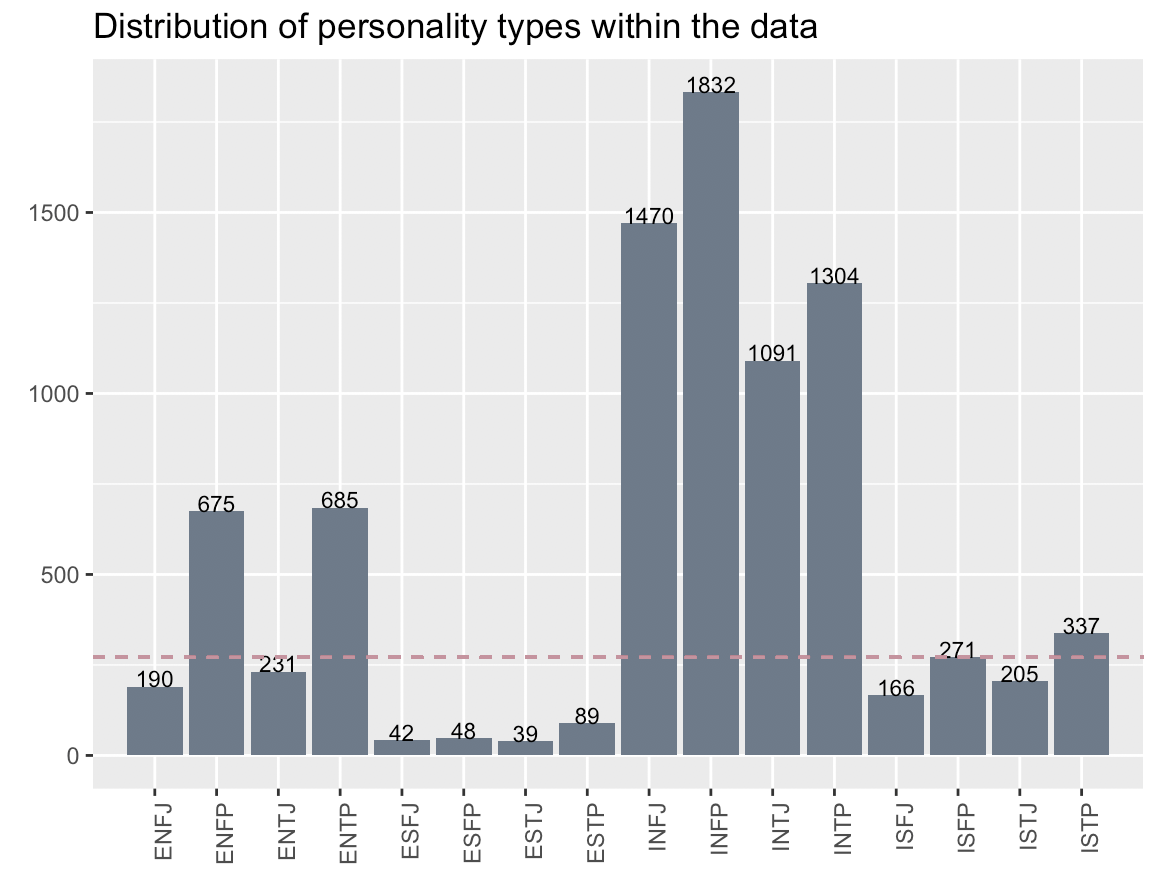
\includegraphics[scale=0.4]{histogram.png}
\caption{Histogram of all personality types including a threshold to indicate types that occurred less than half of the expected times.}
\label{fig:Hist}
\end{figure}

Though the posts rarely contain ``me as an INFP [or any other type]", the posters tend to stay within their own communities  of personality types. This leads to statements such as the following:

\begin{quote}
    ``I think the easiest and most efficient approach is a tarp, jigsaw, and mulcher. But that's just my personal preference. Not all ENTJs are the same." (ENTJ)\\[4pt]
    ``Hey @MsBossyPants are you down for a debate on Ayn Rand vs Marx? Maybe we should talk about our poor Fi? Oh I know- let's try to correlate testing ENTJ with being sociopathic.  :laughing:" (ENTJ)\\[4pt]
    ``The last thing my INFJ friend posted on his facebook before committing suicide the next day. Rest in peace~   http://vimeo.com/22842206" (INFJ)\\[4pt]
    ``a pokemon world  an infj society  everyone becomes an optimist" (INFJ)
\end{quote}

Though the users do not refer to themselves when mentioning the type, they talk about their own personality type much more often than about others, see figure \ref{fig:types}. As this might bias the performance of the model, an unbiased version of the model is included as well. Mentioning one's own personality type and staying within a community of one's own type will however be taken as an important feature for classifying one's personality since it also allows the use of networks for personality prediction.

\begin{figure}
\centering
  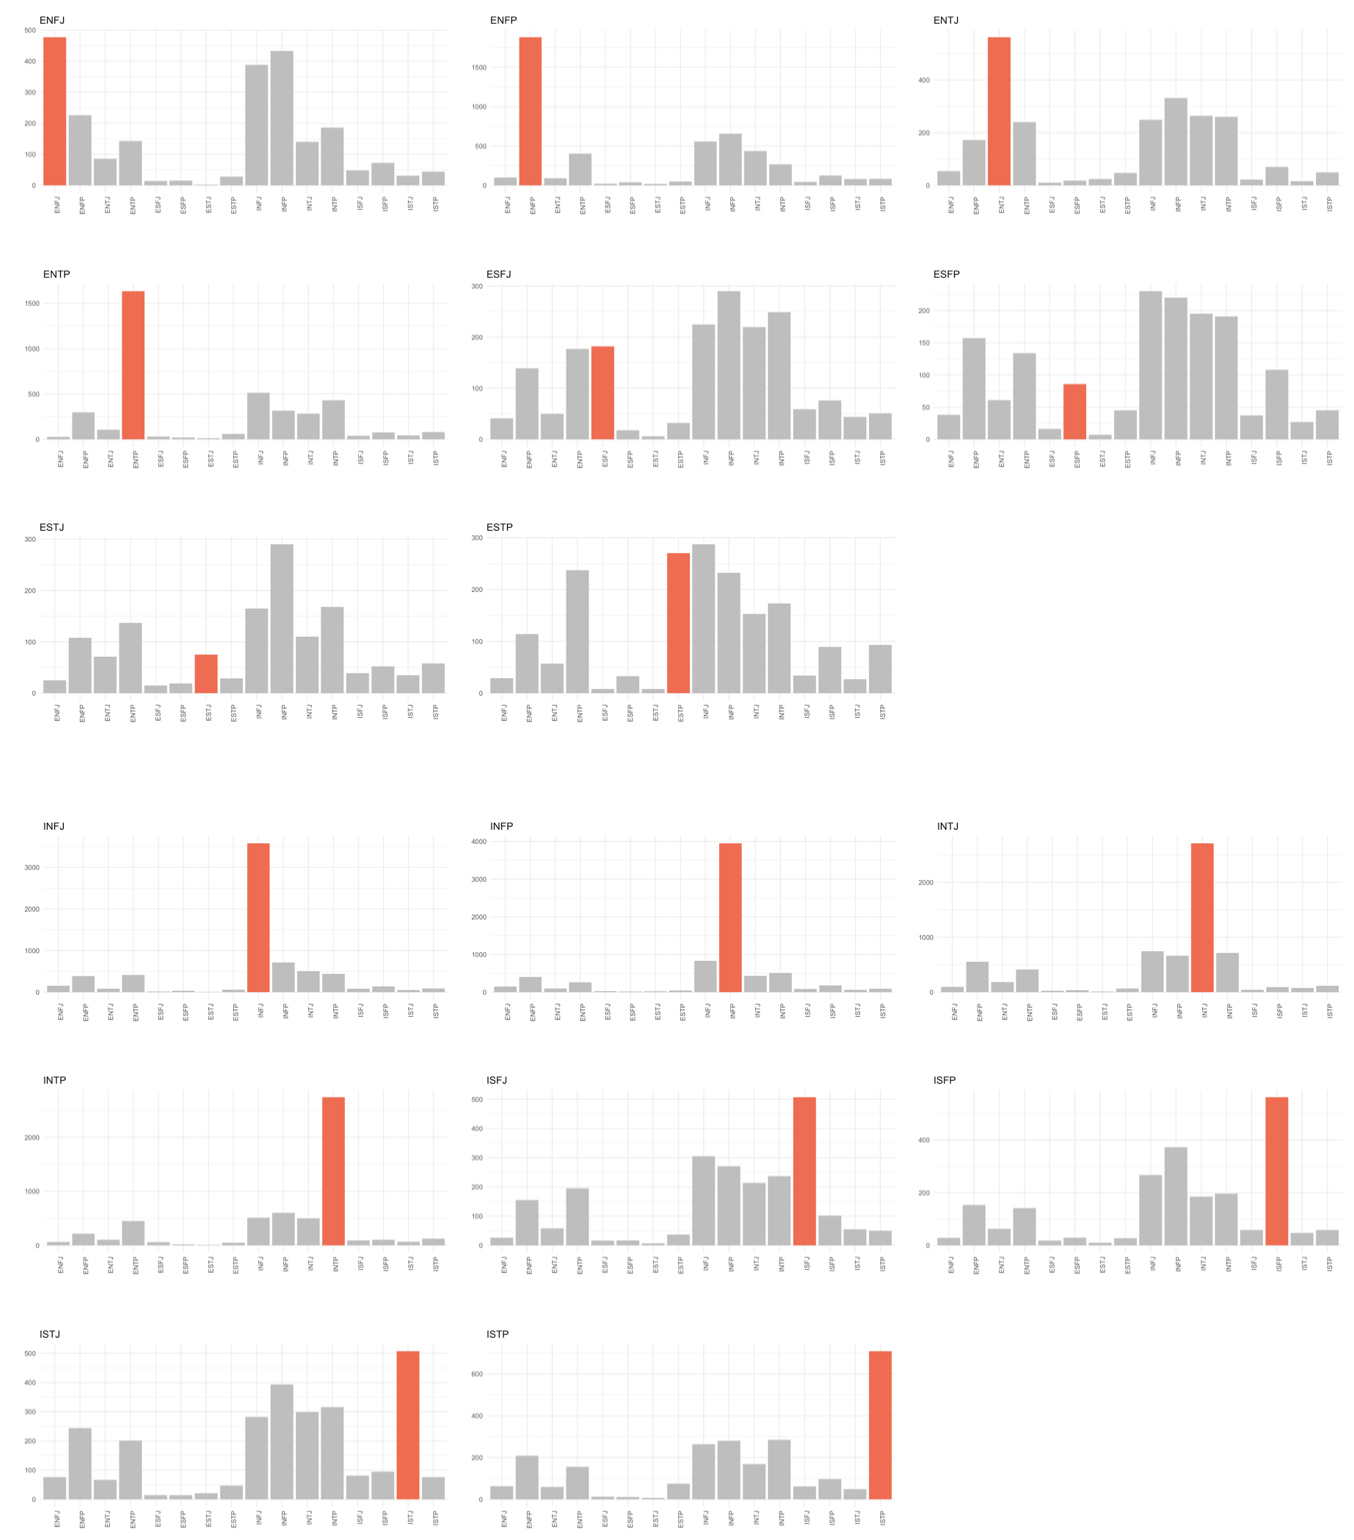
\includegraphics[width=\textwidth]{barchartstype.png}
\caption{Histograms of mentioning any personality type for each of the 16 types.} 
\label{fig:types}
\end{figure}
\section{Methods}
\label{sec:methods}
The prediction of personalities from text is multiple classes classification problem that requires a stable model that can handle many parameters as text produces a vast amount of model parameters. Support Vector Machines (SVMS) are known to produce stable classification results based on text because they hardly overfit. Additionally, text is usually linearly separable, allowing SVMs to determine a margin between categories \cite{carbonell_text_1998}.\\
SVMs are mainly used for supervised classification tasks as present here. For linearly separable data, they do not only separate the data by a line but provide a margin between the data points. The width of the margin is determined by the number of support vectors. These support vectors are the data points that are on the margin or within the margin. Usually, this line is a hyperplane in a high-dimensional space. In this high-dimensional space, the data is then linearly separable. The important mechanism for this is the choice of the kernel function that maps the data to this space.\\
An SVM minimizes the term with quadratic norm ${\frac  {1}{2}}||{\mathbf  w}||_{2}^{2}$ and allows for a soft margin for error $\xi_i$. If there are missclassified samples, the first constraint in equation \ref{eq:1} accounts for the error $\xi_i$ caused by these samples. If there wasn't such error term, the data needed to be linearly seperable with no missclassified samples or the first constraint could never be met. The error is kept low by being part of the objective function in return.\\
\begin{equation}
\begin{array}{rrl}
    \text{min} \quad &{\frac  {1}{2}}||{\mathbf  w}||_{2}^{2}+C\sum _{{i=1}}^{m}\xi _{i} & \\[10pt]
    \text{s.t.} \quad & y_{i} (\langle \mathbf{w,x_{i}} \rangle +b) &\geq 1-\xi _{i}\\
    &1&\leq i \leq m 
\end{array}
\label{eq:1}
\end{equation}

This optimization problem is usually solved using dual formulation with Lagrange multipliers and the KKT, making use of the fact that $w$ can be expressed in terms of the Langrangian multipliers $\alpha$ and $y$.

\begin{equation}
    \begin{array}{cl}
         \max_{\alpha} \quad &\sum _{{i=1}}^{m}\alpha _{i}-{\frac  {1}{2}}\sum _{{i=1}}^{m}\sum _{{j=1}}^{m}\alpha _{i}\alpha _{j}y_{i}y_{j}\langle {\mathbf  x}_{i},{\mathbf  x}_{j}\rangle \\[10pt]
         \text{s.t.} \quad &{\displaystyle 0\leq \alpha _{i}\leq C}\\
         &\sum _{{i=1}}^{m}\alpha _{i}y_{i}=0
    \end{array}
\end{equation}

This yields the classification rule similar to the first constraint in equation \ref{eq:1}:

\begin{equation}
    \begin{array}{c}
        {\displaystyle f(\mathbf {x} )=\operatorname {sgn}(\langle \mathbf {w,x} \rangle +b)=\operatorname {sgn} \left(\sum _{i=1}^{m}\alpha _{i}y_{i}\langle \mathbf {x_{i},x} \rangle +b\right)}
    \end{array}
\end{equation}

The data points that form the margin in the end are the ones where the Lagrangian multipliers are not 0, $\alpha_i \neq 0$.

\paragraph{Pre-processing the data} All texts are pre-processed and cleaned, in particular:
A DocumentTermMatrix of ngrams (3-grams) was created. The SVM ran with n-grams to preserve all sequential information from the posts. After that, stopwords that carry little or no meaning have been removed. All text was then transformed into lowerspace to account for spelling errors. All word or ngram occurrences have been weighted using tf.idf to even out different document lengths:

\begin{equation}
\begin{array}{rl}
    tfidf_t &= f_{t,d} \cdot \log{\frac{N}{df_t}}\\[10pt]
    tfidf_t &= \text{weight of term } t\\
    f_{t,d} &= \text{occurrences of term $t$ in document $d$}\\
    N &= \text{total documents}\\
    d_f &= \text{number of documents containing $t$}
\end{array}
\end{equation}

\paragraph{Features} General quantitative features such as average word length, total words per person and average words per post have been reported.\\
Additionally, the relationship between text and personality allows for linguistic features to be manually extracted.\\
A full set of possibly indicative groups of words and concepts has been added using the word-emotion lexicon by Mohammed \& Turney \cite{mohammad_emotions_2010}. Especially the intuition/sensing dimension can be distinguished by the use of emotions \cite{gjurkovic_reddit:_2018}. Additionally, extraverts post more links \cite{blackwell_extraversion_2017}. They tend to refer more to themselves and use actual self-representation \cite{seidman_self-presentation_2013}. Hence, words like "me", "myself" or "I" resemble the feature "self-representation". Extraverts also communicate more and might thereby use more words in general \cite{seidman_self-presentation_2013}, to explain just a few features used.\\
Following the observations of the data, there will be 6 main models:
One model only uses the features, one SVM uses only the text, one then resembles the two. The \textit{text + features} model is then cleaned by removing one's own personality type and predicting only with the 7 more frequent classes.\\ Hyperparameters were tuned using grid search and a linear kernel. All SVMs were implemented in R using the e1071 library.
\section{Results}
\label{sec:results}

\begin{figure}
\centering
  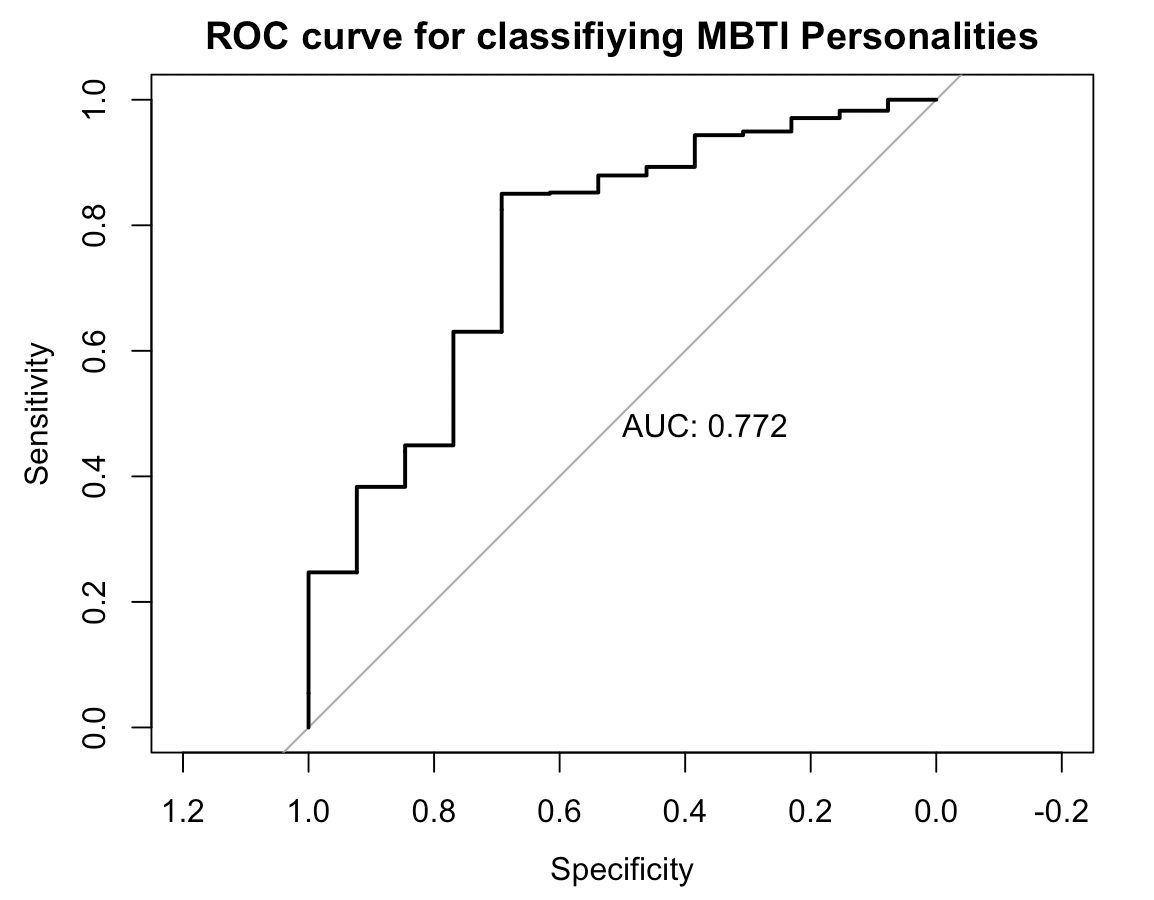
\includegraphics[scale=0.4]{ROC.png}
\caption{Aggregated ROC curve for the multi-class SVM.} %explain multi-class
\label{fig:ROC}
\end{figure}

All SVMs yielded considerably higher results than the baseline. The \textit{text + features} model was able to classify 62\% of people's personality types in the test set correctly, the robust and unbiased model 54\%, see figure \ref{fig:Pred}. This result including a well-shaped ROC curve, figure \ref{fig:ROC}, answers that at least for this dataset the MBTI can be predicted (1). The confusion matrix shows how the prior distribution of personality types influenced the result: most classification errors happened in the more frequent categories among the over-represented introverts. Interestingly, especially the personality types that differ only in one dimension are more often missclassified. This could imply a general validity of the MBTI (2): types that don't have much resemblance in theory are usually not confused here either.
\begin{figure}[b]
\centering
    \begin{subfigure}[b]{.6\textwidth}
      %\centering
      \raggedright
      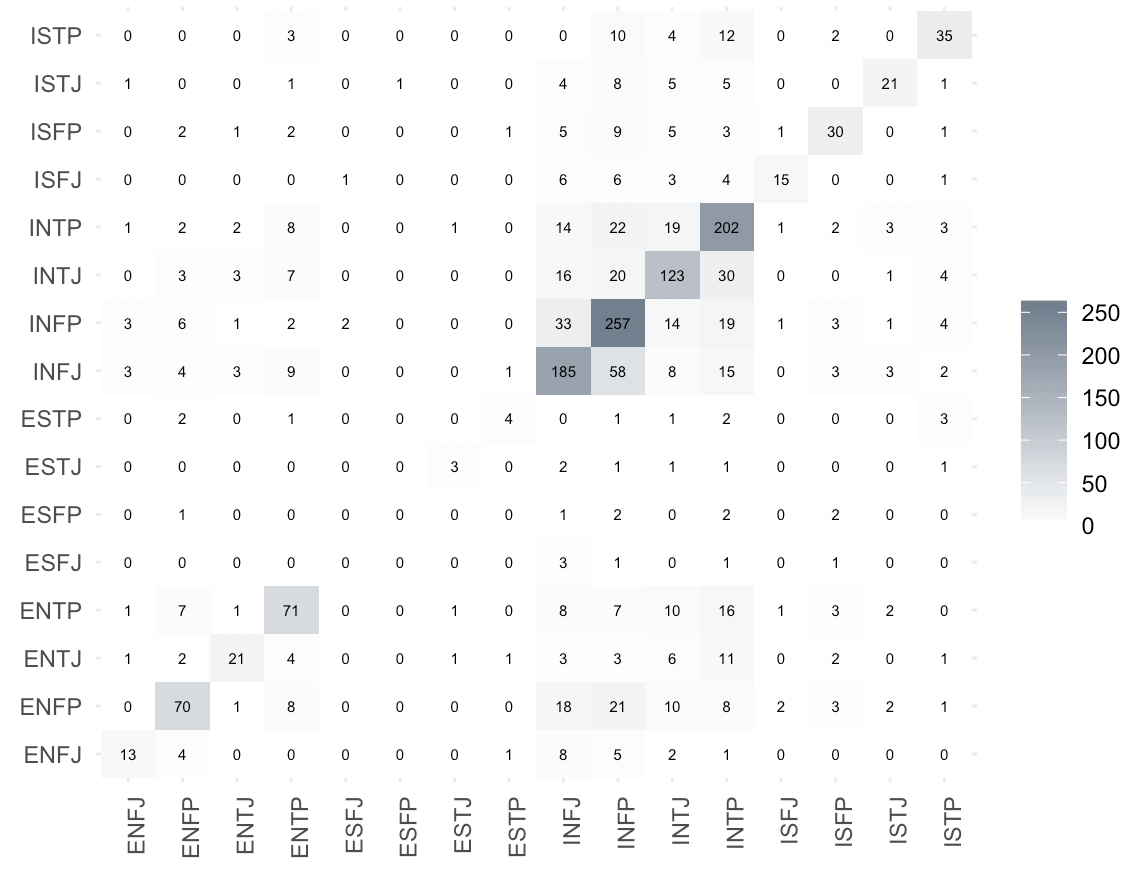
\includegraphics[width=\textwidth]{confusionmatrixlabels.png}
        \caption{Confusion Matrix} %explain more
        \label{fig:Conf}
    \end{subfigure}%
    \quad %spacing between figures
    \begin{subfigure}[b]{.35\textwidth}
        %\begin{table}
        \raggedleft
        \label{tab:Pred}
        \begin{tabular}{ll}
            \hline\noalign{\smallskip}
            \textbf{Model} & \\
            \noalign{\smallskip}\hline\noalign{\smallskip}
            plain features & 0.21 \\
            plain text & 0.56 \\
            text + features & 0.62 \\
            \noalign{\smallskip}\hline\noalign{\smallskip}
            \textit{text + features +} & \\
            unbiased w/o type & 0.46 \\
            robust 7 classes & 0.54 \\
            robust + unbiased & 0.54 \\
            %\noalign{\smallskip}\hline\noalign{\smallskip}
            \noalign{\smallskip}\hline
            \\ \\
        \end{tabular}
        \caption{Prediction accuracy}
        %\end{table}
    \end{subfigure}
    \caption{Prediction results}
    \label{fig:Pred}
\end{figure}
The \textit{plain features} model comes to 21\%. If only the features were used for prediction, they would have to be improved to perform well. As however the personality types are predicted from text, the features may still add some points in accuracy to the model: The text by itself comes to 56\%, with features it is 62\% accurate.\\
This result is unfortunately biased. As predicted, mentioning one's own personality even without referring to oneself has a big impact on the model's performance: if one's own personality type is removed from text, it results in a dropped accuracy of 46\%. If however it is altered to a more robust model with the stable classes, it comes to a promising 54\%. Overall, this supports the notion of the MBTI being predictable here and indicates proof for research question (1).
\section{Discussion}
\label{sec:discussion}
This paper intended to (1) predict MBTI types based on social network posts as done with the Big 5 to then (2) determine if the MBTI is a valid measure for text data. The results show that text can indeed be a good predictor for people's MBTI personality types.
The analysis also showed that similar personality types tend to share communities and hang out with each other. This network effect can be used for future research and implies that network analysis of social media profiles might also predict personality types well.\\
Though the MBTI is not as accepted as the Big 5 Model, it enjoys a high social validity and a broad acceptance in the population. As many people know their MBTI type and are willing to share it online, they grant access to their personal data including their personality type and allow for easily collectible datasets. With the results of this MBTI analysis, one could then derive 4 of the 5 Big Five dimensions as they correlate, giving estimates for a more valid model and easing out the disadvantage of the MBTI.\\
Even if researchers have an interest in these large datasets, the implication that personality can be predicted based on public data such as social media posts is a major threat to a user's data privacy. If the MBTI manages to predict the Big 5, the call for a privacy threat is equally valid for the MBTI. If then the use of data on the Big 5 is heavily restricted \cite{kosinski_facebook_2015}, one could consider doing the same for MBTI data.\\
Such private data has been abused in the past, especially concerning targeted ads during the US-American elections by Cambridge Analytica\cite{krogerus_ich_2018}\footnote{``Cambridge Analytica - The Power of Big Data and Psychographics", https://www.youtube.com/watch?v=n8Dd5aVXLCc, retrieved March 14, 2019.}. The specific manipulation of user's voting preferences raised the question if targeted ads and thus predicting personality is ethical in the first place.\\
Participants seem to be willing to share their data with researchers, e.g. in the most prominent example over 30\% of myPersonality participants voluntarily shared the contents of their Facebook profiles, together with their personality, intelligence, and other psychometric scores \cite{stillwell_mypersonality_2018}. However, one can hardly speak of \textit{informed consent}\cite{fleming_telehealth_2009}, especially because the users will not be able to estimate what could be done with the data. This is why Kosinski et al. propose a consent form with clear intentions on how the data will be used \cite{kosinski_facebook_2015}. This might not solve the overall issue but could be part of a solution to this ethical problem.

\paragraph{Limitations} Not all dimensions delivered equally valid results. Due to the lack of data for the intuition/sensing dimension, a reliable estimate for the correlated agreeableness dimension in the Big 5 cannot be provided using this dataset.\\
Though previous researchers reported lower performances around 0.4 or 0.5 \cite{gjurkovic_reddit:_2018,kosinski_private_2013,kosinski_manifestations_2014} and this model seems to perform fairly well, the fact that the dataset comes from a personality forum cannot be discarded. The personality enthusiasts in that forum will probably be much more aware of their type and identify themselves more with it. This would in return make the type much better identifiable for an algorithm in their expressions and their posts. Thus, the results in this analysis will probably be higher than in a more randomly sampled dataset. In future research, a less specific dataset can shed light on the reliability of predicting the Big 5 using the MBTI and thus on the following privacy issues.


%BibTeX NOT BibLatex!!
% BibTeX users please use one of
%\bibliographystyle{spbasic}      % basic style, author-year citations
\bibliographystyle{spmpsci}      % mathematics and physical sciences
%\bibliographystyle{spphys}       % APS-like style for physics
\bibliography{References}   % name your BibTeX data base

\end{document}

